%作者:汪斐然
%模板用途:模式识别报告
%时间:2021年3月


%这是一份基于《2020-2021模式识别期末提交模板》Word版制作的Latex模板。用于方昱春老师的模式识别课程报告。
%文档中对Latex的各种使用方式都准备了样例并进行备注,包括标题设置、图表添加、文献引用以及字体设置等。
%参考文献格式和Word版存在一定的区别,使用的是IEEETR格式。是IEEE期刊使用的参考文献引用标准。
%参考文献选择使用IEEETR格式的原因在于,可以在文章中对参考文献进行超链接索引。
%希望这份模板可以帮助同学们快速上手Latex,制作漂亮的课程报告;可以在同学们之后的研究学习过程中成为学术论文的参考模板。

%Latex工具:本地编辑平台:TexWorks;在线编辑平台:Overleaf(推荐)

%Latex快速入门教程:
%1、https://muyuuuu.github.io/2018/11/07/Brief-introduction-to-LaTex/
%2、https://liam.page/2014/09/08/latex-introduction/

%Latex快速辅助工具使用说明:
%快速绘制表格工具:https://www.tablesgenerator.com/
%快速生成公式工具:https://mathpix.com/

%%%%%%%%%%%%%%%%%%%%%%%%%%%%%环境配置%%%%%%%%%%%%%%%%%%%%%%%%%%%%%%%%%%

\documentclass{article}
\usepackage[UTF8]{ctex}
\usepackage[left=3.18cm,right=3.18cm,top=2.54cm,bottom=2.54cm]{geometry}
\geometry{a4paper}

%附录包
\usepackage{appendix} 
\usepackage{listings}
\usepackage{cite}
%代码格式
\usepackage{xcolor}
\lstset{
    numbers=left, 
    numberstyle= \tiny, 
    keywordstyle= \color{ blue!70},
    commentstyle= \color{red!50!green!50!blue!50}, 
    frame=shadowbox, % 阴影效果
    rulesepcolor= \color{ red!20!green!20!blue!20} ,
    escapeinside=``, % 英文分号中可写入中文
    xleftmargin=2em,xrightmargin=2em, aboveskip=1em,
    framexleftmargin=2em
} 
\usepackage{algorithm}
\usepackage{algpseudocode}
\renewcommand{\algorithmicrequire}{\textbf{Input:}}  % Use Input in the 
\renewcommand{\algorithmicensure}{\textbf{Output:}} % Use Output in the 

%数学
\usepackage{amsmath}
\usepackage{amsthm}

%图片
\usepackage{graphicx} %添加图片

%字体、格式设置
\usepackage{subfigure}
\usepackage{float}
\renewcommand{\vec}[1]{\boldsymbol{#1}} % 生产粗体向量,而不是带箭头的向量
\usepackage{amssymb}
\usepackage{booktabs} % excel导出的大表格
\usepackage{hyperref}
\usepackage{titlesec}%设置字体的包
%可选字体:
% \noindent 中文字体(默认宋体)\\
% \fangsong 中文字体(仿宋) \songti 中文字体(宋体) \lishu 中文字体(隶书) \heiti 中文字体(黑体)\\
% \CJKfamily{zhkai} 中文字体(楷书) \CJKfamily{zhyou} 中文字体(幼圆) \CJKfamily{zhyahei} 中文字体(微软雅黑)\\

%调整图表标题的字体样式
\usepackage{caption}
\captionsetup{font={small,bf}} 

%新定义
\newtheorem{definition}{定义} %中文
\newtheorem{lemma}{引理}
\newtheorem{theorem}{定理}
\DeclareMathOperator{\Ima}{Im}%定义新符号
\DeclareMathOperator{\Rank}{rank}%定义求秩算子

\usepackage{pdfpages}


%设置标题,作者
\title{\textbf{基于XGBoost与SVM的网络入侵检测系统:以UNSW-NB15数据集为例}}
\author{
王宇飞(22122850)
}

%%%%%%%%%%%%%%%%%%%%%%%%%%%%%%%正文%%%%%%%%%%%%%%%%%%%%%%%%%%%%%%%%%%
%\songti(宋体)设置全文字体,可改为\heiti(黑体),\fangsong(仿宋)
\begin{document} \songti

% \centerline{\heiti\zihao{2}{上海大学2024 $ \sim $ 2025学年}}
\vspace{10bp}
\centerline{\heiti\zihao{2}{课程报告成绩评价表}}

\vskip 2cm

\begin{flushleft}
	\zihao{3}
	{\heiti{课程名称:}}      
	{\heiti\underline{\quad\textbf{《模式识别》}\quad}}
        {\heiti{课程编号:}}      
	{\heiti\underline{\quad\textbf{08306089}\hspace{1cm}}}   
                \\
	\vspace{20bp}
	{\heiti{ {报告名称:}}}      
	{\heiti\underline{\hspace{2.8cm}\textbf{}\hspace{8.8cm}}}              
                \\
	\vspace{20bp}
	{\heiti{{姓}\quad\quad{名:}}}      
	{\heiti\underline{\quad\quad\quad\quad\textbf{哇}\quad\quad\quad\quad}}
        {\heiti{{学}\quad\quad{号:}}}      
	{\heiti\underline{\quad\quad\quad\textbf{}\quad\quad\quad\quad}} 
                \\
        \vspace{20bp}
	{\heiti{ {报告评语:}}} 
                \\
        \vspace{15bp}
        \fbox{%
            \parbox{1.04\textwidth}{%
                \begin{center}
                    \\\quad 
                    \\\quad 
                \end{center}
                }%
            }
        
        \vspace{20bp}
	{\heiti{{报告成绩:}}} 
\\
\vspace{5bp}
\begin{table}[htbp]
\setlength{\tabcolsep}{0.37cm}
\begin{tabular}{|cl|cl|cll|c|}
\hline
\multicolumn{2}{|c|}{方案设计(20分)}                                                                                                                      & \multicolumn{2}{c|}{验收(20分)}                                                                                                                         & \multicolumn{3}{c|}{书面报告(60分)}                                                                                                                      & \multirow{2}{*}{总分}   \\ \cline{1-7}
\multicolumn{1}{|c|}{\begin{tabular}[c]{@{}c@{}}可行性\\ (10分)\end{tabular}} & \multicolumn{1}{c|}{\begin{tabular}[c]{@{}c@{}}创新性\\ (10分)\end{tabular}} & \multicolumn{1}{c|}{\begin{tabular}[c]{@{}c@{}}规范性\\ (10分)\end{tabular}} & \multicolumn{1}{c|}{\begin{tabular}[c]{@{}c@{}}演示效果\\ (10分)\end{tabular}} & \multicolumn{1}{c|}{\begin{tabular}[c]{@{}c@{}}规范性\\ (20分)\end{tabular}} & \multicolumn{1}{c|}{\begin{tabular}[c]{@{}c@{}}完整性\\ (20分)\end{tabular}} & \multicolumn{1}{c|}{\begin{tabular}[c]{@{}c@{}}科学性\\ (20分)\end{tabular}} &                       \\ \hline
\multicolumn{1}{|l|}{}                                                    &                                                                          & \multicolumn{1}{l|}{}                                                    &                                                                           & \multicolumn{1}{l|}{}                                                    & \multicolumn{1}{l|}{}                                                    &           \rule{0pt}{3\normalbaselineskip}                                                               & \multicolumn{1}{l|}{} \\ \hline

\end{tabular}
\end{table}

\end{flushleft}

\vspace{20bp}
\leftline{\heiti\zihao{3}{任课教师:}}
\vspace{20bp}
\leftline{\heiti\zihao{3} {评阅日期:     \quad\quad\quad     年  \quad\quad  月  \quad\quad  日         }} %调用封面文件
% 插入封面

\date{}
\maketitle


%%%%%%%%%%%%%%%%%%%%%%摘要%%%%%%%%%%%%%%%%%%%%%%%%%%%%%
%由摘要和关键词两部分组成
\begin{center}
\setlength{\textwidth}{15cm}
\parbox{\textwidth}{
\textbf{摘要:}针对网络入侵检测中高维流量\cite{ref1}数据带来的计算效率低、复杂攻击识别困难等问题,本研究提
出基于XGBoost与非线性缩放支持向量机(SVM)的混合检测模型。基于UNSW-NB15现代化流量数据集,通过XGBoost特征
选择算法提取20个关键特征,实现特征空间压缩至原数据集的47\%,显著降低
计算复杂度。在二分类(正常/异常)和多分类任务中,模型分别取得85.81\%与69.86\%的准确率,
F1值达88.28\%和72.10\%,实验表明,与传统检测方法相比,该方法在
在优化计算效率的同时,依旧保持了较优的检测准确率。

% \newline
%   \textbf{关键词:}图像分类, K近邻, 支持向量机, 数据增强
  }
\end{center}

%%%%%%%%%%%%%%%%%%%%%%目录%%%%%%%%%%%%%%%%%%%%%%%%%%%%%
% \newpage
% \tableofcontents
% \newpage
%%%%%%%%%%%%%%%%%%%%%%%%%%%%%%%%%%%%%%%%%%%%%%%%%%%%%%%%
%一级标题
\section{引言}
%%%%%%%%%%%%%%%%%%%%%%%%%%%
%二级标题
\subsection{研究背景}
随着信息技术的飞速发展,网络已成为现代社会不可或缺的一部分。然而,伴随而来的网络安全问题日益复杂且严峻。作为
网络安全防护的重要组成部分
,网络入侵检测系统(NIDS)在保障网络安全方面扮演着至关重要的角色。传统的入侵检测方法通常依赖基于规则的
模式识别,但面对复杂多变的攻击模式时,这些方法往往显得力不从心。特别是在处理高维流量数据时,传统方法面临
计算效率低、误报率高以及对复杂攻击识别困难等问题,这些都严重制约了其在实际应用中的普适性和有效性。

\subsection{方法引入}
近年来,随着机器学习技术的不断进步,尤其是基于集成学习和支持向量机(SVM)的方法逐渐被引入到网络
入侵检测领域。这些方法能够自动学习流量特征,从而优化检测精度与计算效率。同时XGBoost(Extreme Gradient
 Boosting)作为一种高效的梯度提升算法,以其优秀的特征选择能力和处理高维数据的优势,已在多个领域得到广
 泛应用。而SVM则因其出色的分类性能和在处理非线性问题时的强大能力,成为解决网络入侵检测任务的重要工具。

\subsection{论文概述}
本研究提出了一种基于XGBoost与非线性SVM的混合检测模型,旨在解决现有方法在高维流量数据下计算效率低
和复杂攻击识别困难的问题。首先,利用UNSW-NB15现代化流量数据集,本研究应用XGBoost算法进行特征选择,
提取出20个关键特征,将特征空间压缩至原数据集的47\%,显著降低了计算复杂度。接着,基于压缩后的特征空间
,进行二分类(正常/异常)和多分类任务,从而在提升检测效率的同时,保持了较优的准确率和F1值。


%%%%%%%%%%%%%%%%%%%%%%%%%%%%%%%%%%%%%%%%%%%%%%%%%%%%%%%%


\section{数据集与预处理}
%%%%%%%%%%%%%%%%%%%%%%%%%%%
\subsection{UNSW-NB15数据集}
UNSW-NB15数据集是由澳大利亚新南威尔士大学堪培拉分校(UNSW Canberra)的网络靶场实验室
(Cyber Range Lab)使用IXIA PerfectStorm工具生成的。该数据集旨在模拟现代网络环境中的正常活
动和合成攻击行为,从而为网络入侵检测研究提供高质量的实验数据。通过Tcpdump工具捕获了100 GB的原始
网络流量数据(如Pcap文件),并进一步处理生成了包含多种攻击类型和正常流量的结构化数据集。在这项工作中,UNSW-NB15 
数据集中共有 257,673 个
数据实例,其中包括 175,341 个训练数据实例和 82,332 个测
试数据实例。
\subsubsection{数据集分类情况}
UNSW-NB15数据集涵盖了一种正常流量类型和九种主要的攻击类型,包括Fuzzers、Analysis、Backdoors、DoS(拒绝服务攻击)
、Exploits、Generic、Reconnaissance(侦察攻击)、Shellcode和Worms。这些攻击类型覆盖了广泛的网络威
胁,能够有效支持入侵检测系统的训练与评估。
\begin{table}[H]
  \caption{UNSW-NB15数据集中的标签及其含义}
  \label{table:sample} % 将label放在caption之后
  \begin{center}
    \resizebox{\textwidth}{!}{  % 按页面宽度缩放表格
  \begin{tabular}{|l|l|l|} % 使用 r 表示右对齐
\hline
ID & Type           & Description                                                                                                            \\ \hline
1  & Normal         & Natural transaction data.                                                                                              \\ \hline
2  & Analysis       & An attack to invade web applications through emails ports or web scripts.                                              \\ \hline
3  & Backdoor       & A covert attempt to circumvent normal authentication measures or other processes by allowing for secure remote access. \\ \hline
4  & DoS            & A malicious attempt to disrupt the computer resources by attacking memory.                                             \\ \hline
5  & Exploits       & An instruction to take advantage of bugs or errors caused by unintentional behavior on the network.                    \\ \hline
6  & Fuzzers        & An attack to crash the system by inputting a lot of random data.                                                       \\ \hline
7  & Generic        & A technique to clash the block-cipher configuration by using hash functions.                                           \\ \hline
8  & Reconnaissance & A probe to evade network security controls by collecting relevant information.                                         \\ \hline
9  & Shellcode      & A piece of code that is executed to exploit software vulnerabilities.                                                  \\ \hline
10 & Worms          & A set of virus code which can add itself to computer system or other programs.                                         \\ \hline
\end{tabular}
    }
\end{center}
\end{table}
\subsubsection{数据集特征情况}
本数据集的257,673项数据中,共含有49个特征(包含类别标签),其中所有特征被分为 6 组,
包括流量、基础、内容、时间、附加生成和标记特征。特
别地,特征 1 至 35 代表从数据包中集成收集的信息。附
加生成的特征进一步分为通用特征和连接特征两部分。特
征 36 至 39 被视为连接特征,而特征 40 至 47 被视为
通用特征。特征 48 至 49 为标记特征。
\begin{table}[H]
  \caption{UNSW-NB15数据集中的特征}
  \label{table:feature} % 将label放在caption之后
  \begin{center}
    \resizebox{\textwidth}{!}{  % 按页面宽度缩放表格
    \begin{tabular}{|l|l|l|l|l|l|l|l|}
      \hline
      No. & Name   & No. & Name          & No. & Name                & No. & Name                \\ \hline
      1   & srcip  & 14  & service       & 27  & Sjit                & 40  & ct\_ftp\_cmd        \\ \hline
      2   & sport  & 15  & Sload         & 28  & Djit                & 41  & ct\_srv\_src        \\ \hline
      3   & dstip  & 16  & Dload         & 29  & Stime               & 42  & ct\_srv\_dst        \\ \hline
      4   & dsport & 17  & Spkts         & 30  & Ltime               & 43  & ct\_dst\_ltm        \\ \hline
      5   & proto  & 18  & Dpkts         & 31  & Sintpkt             & 44  & ct\_src\_ ltm       \\ \hline
      6   & state  & 19  & swin          & 32  & Dintpkt             & 45  & ct\_src\_dport\_ltm \\ \hline
      7   & dur    & 20  & dwin          & 33  & tcprtt              & 46  & ct\_dst\_sport\_ltm \\ \hline
      8   & sbytes & 21  & stcpb         & 34  & synack              & 47  & ct\_dst\_src\_ltm   \\ \hline
      9   & dbytes & 22  & dtcpb         & 35  & ackdat              & 48  & attack\_cat         \\ \hline
      10  & sttl   & 23  & smeansz       & 36  & is\_sm\_ips\_ports  & 49  & Label               \\ \hline
      11  & dttl   & 24  & dmeansz       & 37  & ct\_state\_ttl      &     &                     \\ \hline
      12  & sloss  & 25  & trans\_depth  & 38  & ct\_flw\_http\_mthd &     &                     \\ \hline
      13  & dloss  & 26  & res\_bdy\_len & 39  & is\_ftp\_login      &     &                     \\ \hline
  \end{tabular}
    }
  \end{center}
\end{table}
\subsubsection{数据分布情况}
由图\ref{fig:combined}可以发现,数据集中各类别的条目数量分布并不均衡,这有可能导致模型在训练和测试过程中对于少数类别的识别效果不佳。
因此,在训练与评估模型时,需要采取一些策略来处理数据集中的类别不平衡问题。
\begin{figure}[H]
  \centering
  \begin{minipage}[b]{0.45\textwidth}
      \centering
      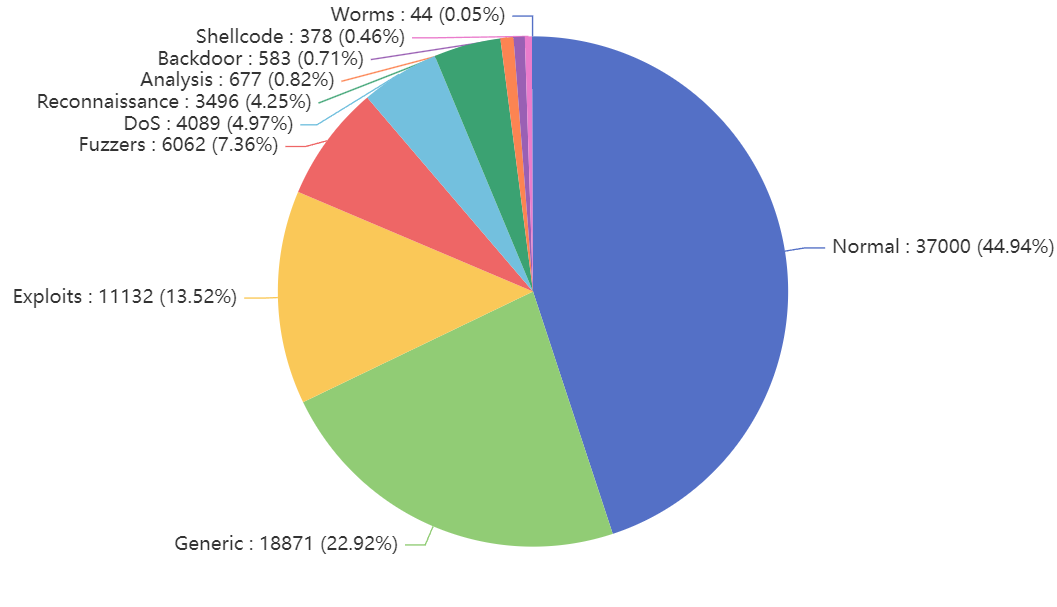
\includegraphics[width=\textwidth]{./png/acc2.png}
      % \caption{测试集攻击分类占比情况}
      \label{fig:test_set}
  \end{minipage}
  \hspace{0.05\textwidth}  % 图像之间的水平间距
  \begin{minipage}[b]{0.45\textwidth}
      \centering
      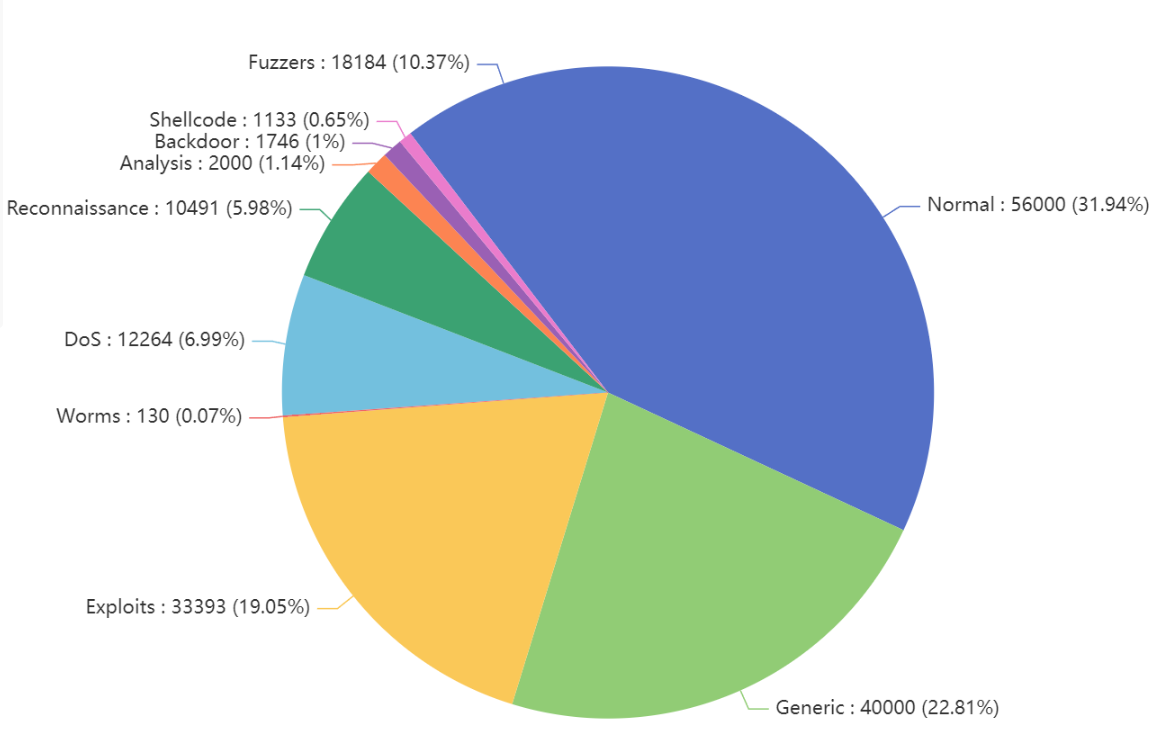
\includegraphics[width=\textwidth]{./png/acc1.png}
      % \caption{训练集攻击分类占比情况}
      \label{fig:train_set}
  \end{minipage}
  \caption{训练集与测试集攻击分类占比情况}
  \label{fig:combined}
\end{figure}

\subsection{数据预处理}

\subsubsection{数据完整度检验}
由于数据量过大,为了提高数据处理效率,我们首先对数据集进行了数据完整性检验。如图\ref{fig:full}所示,
service列出现超过半数的数据缺失,因此我们选择从数据集中移除该列数据,防止对后续的模型训练造成影响。
\begin{figure}[htpb]
  \centering
  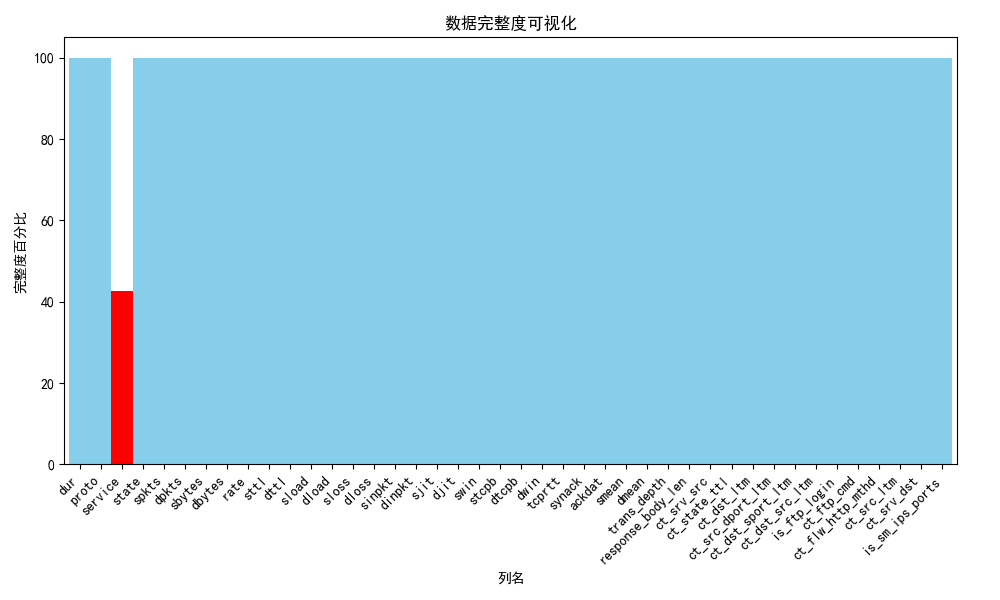
\includegraphics[width=0.9\textwidth]{./png/full.png}
  \caption{数据完整性}
  \label{fig:full}
\end{figure}
\subsubsection{字符串标签列处理}
在数据集中,有一些列的数据类型为字符串,例如proto、state等。
为了方便后续的模型训练,我们选择独热编码将这些字符串标签列进行了数值化处理。
独热编码通过创建新列来处理分类列,这些新列映射到其
中的不同值的数量。每个新列代表一个单独的独特类别。
它将 1 分配给与类别位置在原始列中匹配的位置,其余
部分为 0。
\subsubsection{数据标准化}

首先,我们计算了原始数据的偏度值。偏度是衡量数据分布对称性的一种统计量。
若偏度值接近0,则表示数据分布接近正态分布;若偏度值显著大于0或小于0,则说明数据分布偏向右侧或左侧。
由图\ref{fig:skew}可知,原始数据的偏度值存在显著的偏斜,显示出非常强烈的右偏分布,
这些强烈的偏斜可能会对基于正态分布假设的模型(如线性回归)产生负面影响,因此需要进行标准化处理。

为了解决数据的偏斜问题,我们对数据进行了对数转换:
\begin{equation}
 F(x)= \log _{10} x
\end{equation}

对数转换是一种常用的标准化方法,它可以有效地减少正偏分布的影响,并使数据趋向正态分布。
通过对原始数据进行对数转换后,数据偏度值明显降低,大多数特征的偏度接近零,表示数据分布趋向正态,显著改善了该特征的分布。
\begin{figure}[H]
  \centering
  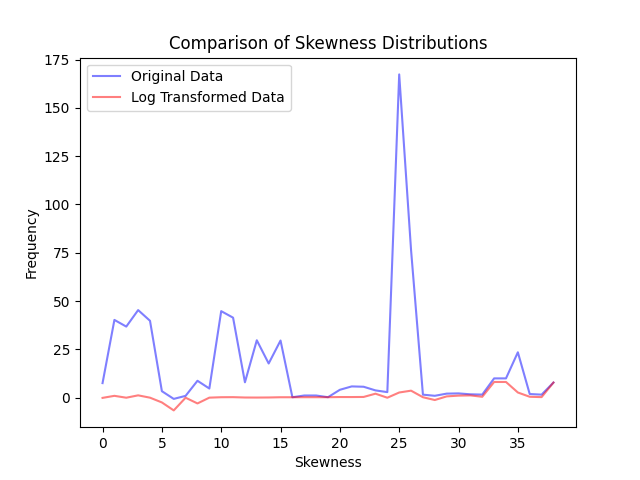
\includegraphics[width=0.7\textwidth]{./png/skewness.png}
  \caption{数据偏度量}
  \label{fig:skew}
\end{figure}

%%%%%%%%%%%%%%%%%%%%%%%%%%%%%%%%%%%%%%%%%%%%%%%%%%%%%%%%


\section{模型构建}
\subsection{特征选择}
对于机器学习算法而言,特征数量的
增加会显著延长学习入侵任务所需的训练时间[jan13]。因此,
特征选择对训练和分类过程都有益处,它能有效减少所
需处理的数据量、降低问题的维度以及减少内存和 CPU 
的使用。UNSW-NB15考虑了 49 多个特征,但其中某些
特征在异常检测中可能并不重要[jan],基于此本文采用
基于XGBoost的特征重要性排序的特征选择方法。
\subsubsection{XGBoost技术}
XGBoost(Extreme Gradient Boosting)是一种基于梯度提升算法的集成学习方法,通过构建多个决策树来进行回归和分类任务。
该方法在特征提取中的应用表现出显著优势,特别是在高维数据和大规模数据集上,能够自动学习数据中的复杂特征并进行高效建模。
XGBoost的关键技术包括梯度提升树、正则化、并行化和缺失值处理等,这些都为特征提取提供了强大的支持。

XGBoost的核心是梯度提升算法(Gradient Boosting)。梯度提升通过构建一系列弱分类器(通常是决策树)
来提高模型的准确性。每一棵新树都在前一棵树的基础上进行训练,调整预测误差。XGBoost的目标是最小化以下目标函数:
XGBoost的目标是最小化以下目标函数:
\begin{equation}
L(\Theta) = \sum_{i=1}^{N} \mathcal{L}(y_i, \hat{y}_i) + \Omega(f_t)
\end{equation}

XGBoost的训练过程采用了贪心算法和梯度下降的方法。对于每一轮迭代,XGBoost通过计算梯度
和二阶导数来更新每一棵树的叶子节点权重,优化目标函数。训练过程大致可以通过以下伪代码描述:
\begin{algorithm}[H]
  \caption{XGBoost算法步骤}
  \begin{algorithmic}[1]
    \Require Training data $\{(x_i, y_i)\}_{i=1}^{N}$, initial model $f_0(x)$, number of boosting rounds $T$, learning rate $\eta$, regularization parameters $\lambda, \gamma$
    \Ensure Final model $f_T(x)$
    \State Initialize model: $f_0(x) = 0$
    \For{$t = 1$ \textbf{to} $T$}
      \State Compute residuals: $r_i^{(t)} = -\frac{\partial \mathcal{L}(y_i, f_{t-1}(x_i))}{\partial f_{t-1}(x_i)}$ for all $i$
      \State Fit a new decision tree $h_t(x)$ to the residuals $\{r_i^{(t)}\}_{i=1}^{N}$
      \State Compute the optimal tree weights: $\rho_t = \arg\min_{\rho} \sum_{i=1}^{N} \mathcal{L}(y_i, f_{t-1}(x_i) + \rho h_t(x_i)) + \Omega(h_t)$
      \State Update the model: $f_t(x) = f_{t-1}(x) + \eta \rho_t h_t(x)$
      \State Prune the tree $h_t(x)$ if necessary (based on regularization $\lambda$ and $\gamma$)
    \EndFor
    \Return $f_T(x)$
  \end{algorithmic}
\end{algorithm}
在特征提取过程中,XGBoost通过学习数据的分裂点,自动捕捉特征之间的复杂关系。在每次训练迭代中,
XGBoost通过选择一个特征来进行决策树的最优分裂,从而逐步提高模型的预测精度。训练完成后,XGBoost会为每个特征计算
一个“特征重要性分数”(Feature Importance, FI),该分数衡量了特征在模型中的重要性。

在本研究中,我们采用了FI-Gain度量作为评估特征重要性的标准。FI-Gain度量反映了特征在决策树中分裂时对目标函数的贡献,
具体来说,它表示某一特征在分裂时所带来的目标函数减少的程度。简而言之,分裂增益(Gain)反映了该特征在减少预测误差方面的贡献。
因此,XGBoost通过计算每个特征在树的每次分裂中对损失函数的影响,评估并确定特征的重要性。根据分数,选出了前20个重要特征训练模型,
如表\ref{table:feature1}所示。
\begin{table}[H]
  \caption{XGBoost模型中特征重要性排名}
  \label{table:feature1} % 将label放在caption之后
  \begin{center}
    \resizebox{\textwidth}{!}{  % 按页面宽度缩放表格

\begin{tabular}{|l|l|l|l|}
\hline
Feature             & XGBoost\_Importance & Feature             & XGBoost\_Importance \\ \hline
sttl                & 4506.0146484375     & swin                & 123.2380828857422   \\ \hline
is\_sm\_ips\_ports  & 4040.569091796875   & synack              & 106.19803619384766  \\ \hline
ct\_state\_ttl      & 2723.21484375       & dload               & 93.36001586914062   \\ \hline
ct\_srv\_dst        & 358.7242736816406   & dmean               & 84.627197265625     \\ \hline
dttl                & 285.3583374023437   & dbytes              & 68.91485595703125   \\ \hline
dpkts               & 168.32664489746094  & trans\_depth        & 68.65630340576172   \\ \hline
ct\_dst\_sport\_ltm & 164.348876953125    & ct\_srv\_src        & 65.3878402709961    \\ \hline
sbytes              & 152.1552734375      & ct\_dst\_src\_ltm   & 57.510398864746094  \\ \hline
proto               & 135.38369750976562  & sloss               & 47.56684112548828   \\ \hline
smean               & 132.0811767578125   & ct\_flw\_http\_mthd & 46.42452239990234   \\ \hline
\end{tabular}

    }
\end{center}
\end{table}
\subsection{SVM模型}
支持向量机(SVM)是一种常用的监督学习算法,特别适用于高维空间中的分类任务,
因此常被用于入侵检测。在SVM模型中,核函数起着关键作用,它将数据从低维空间映射到高维空间,
从而使得线性不可分的数据变得可分。常见的核函数包括线性核、多项式核、径向基核(RBF)、高斯核、拉普拉斯核和S型核等[7]。

由于入侵检测任务的数据集通常较大,训练和测试的时间开销成为需要考虑的重要因素。在选择核函数时
,除了考虑模型的准确性,还需要综合考虑计算时间。因为径向基核(RBF)优异的性能,
能够在准确性和计算效率之间取得良好的平衡,被我们选为SVM模型的核函数。
\begin{figure}[H]
  \centering
  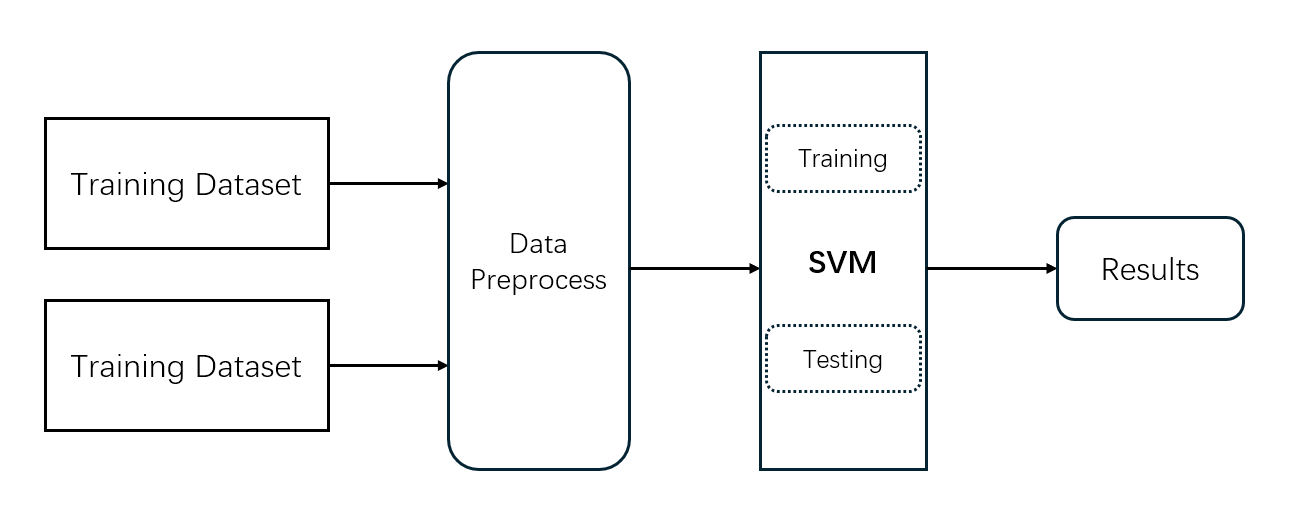
\includegraphics[width=0.8\textwidth]{./png/model.png}
  \caption{采用SVM模型的入侵检测流程图}
  \label{fig:svm}
\end{figure}
\subsection{模型评估}

在本研究中,我们使用混淆矩阵(Confusion Matrix)来评估模型的性能。混淆矩阵是通过将预测结果与真实标签进行对比,来衡量模型分类效果的工具。通过混淆矩阵可以计算出多个评价指标,例如准确率(Accuracy)、精确度(Precision)、召回率(Recall)、F1 分数(F1-Score)等。

给定混淆矩阵:

\[
\begin{bmatrix}
    TN & FP \\
    FN & TP
\end{bmatrix}
\]

其中,$TN$ 是真正例(True Negatives)、$FP$ 是假正例(False Positives)、$FN$ 是假负例(False Negatives)、$TP$ 是真正例(True Positives)。

根据混淆矩阵,定义了以下常见的评价指标:

1. 准确率 (Accuracy)

   准确率表示模型正确分类的样本所占的比例,计算公式为:

   \[
   \text{Accuracy} = \frac{TP + TN}{TP + TN + FP + FN}
   \]

   其中,$TP + TN$ 是正确预测的数量,$FP + FN$ 是错误预测的数量。

2. 精确度 (Precision)

   精确度度量的是模型预测为正类的样本中,真实为正类的比例,计算公式为:

   \[
   \text{Precision} = \frac{TP}{TP + FP}
   \]

   高精确度意味着模型很少将负类误判为正类。

3. 召回率 (Recall)

   召回率度量的是实际为正类的样本中,模型正确预测为正类的比例,计算公式为:

   \[
   \text{Recall} = \frac{TP}{TP + FN}
   \]

   高召回率意味着模型能捕捉到大部分的正类样本。

4. F1 分数 (F1-Score)

   F1 分数是精确度和召回率的调和平均值,综合考虑了假正例和假负例的影响,计算公式为:

   \[
   \text{F1-Score} = \frac{2 \times \text{Precision} \times \text{Recall}}{\text{Precision} + \text{Recall}}
   \]

   F1 分数越高,说明模型的分类性能越好,尤其是在精确度和召回率之间取得良好的平衡。

5. 训练时间
   训练时间是评估模型性能的重要指标之一,它反映了模型训练所需的时间开销。在实际应用中,训练时间的长短直接影响了模型的实用性和可扩展性。



\section{实验结果}
\subsection{二分类实验结果}
\begin{table}[H]
  \caption{二分类下性能对比}
  \label{table:feature_selection_performance}
  \centering
  \begin{tabular}{lccccc}
    \toprule
    特征子集          & Accuracy & Recall & Precision & F1 Score & Time/s \\ \midrule
    42-Orginal-Features & 0.8555   & 0.9733 & 0.8079    & 0.8806   & 72.36  \\
    20-XGB-Features     & 0.8581   & 0.9677 & 0.8077    & 0.8828   & 63.65  \\ \bottomrule
  \end{tabular}
\end{table}
实验结果表明,基于XGBoost的特征选择方法在保持较高分类性能的同时,显著减少了特征数量和计算时间。
使用20个XGBoost特征子集的模型准确率达到85.81\%,略高于使用全部42个原始特征的85.55\%,
同时运行时间从72.36秒减少至63.65秒,显著提升了计算效率。尽管召回率从97.33\%略微下降
至96.77\%,但F1分数从88.06\%提升至88.28\%,表明该方法在平衡精确率和召回率方面表
现更好。总体而言,XGBoost特征选择方法在降低数据维度和提升模型效率方面具有显著优势,适用于实际网络入侵检测系统的部署。
\subsection{多分类实验结果}

\begin{table}[H]
  \caption{多分类下性能对比}
  \label{table:feature_selection_performance_m}
  \centering
  \begin{tabular}{lccccc}
    \toprule
    特征子集          & Accuracy & Recall & Precision & F1 Score & Time/s \\ \midrule
    42-Orginal-Features     & 0.6958   & 0.6958 & 0.7821    & 0.7193   & 507.35  \\    
    20-XGB-Features    & 0.6986   & 0.6986 & 0.7793    & 0.7210   & 438.76  \\\bottomrule 

  \end{tabular}
\end{table}
在多分类任务中,除了训练时间有显著提升外,其他性能指标的变化不大。说明原始数据集中确实存在较多干扰特征。同时根据\ref{fig:class},
不同类别分类正确率有较大偏差,说明数据集中存在类别不平衡问题,符合前文对于数据集的分析,这也是模型性能提升的瓶颈之一。

\begin{figure}[htpb]
  \centering
  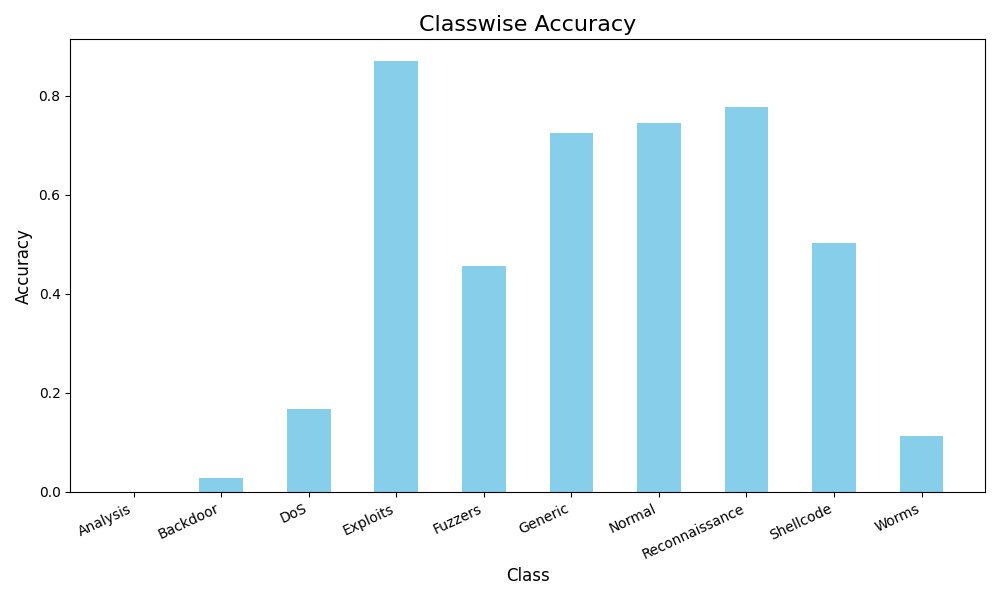
\includegraphics[width=0.8\textwidth]{./png/classwise_accuracy.png}
  \caption{不同类别分类正确率}
  \label{fig:class}
\end{figure}

\subsection{与其他模型性能对比}
在二分类情况下,Moustafa和Slay曾使用朴素贝叶斯(NB)、决策树(DT)、人工神经网络(ANN)、逻辑回归(LR)以及期望最大化聚类(EM)等方法对UNSW-NB15
数据集进行分类实验,结果如表\ref{table:compare1}所示。可以看到本文提出的基于XGBoost-SVM的方法在上均优于其他方法。

Sydney M. Kasongo  and Yanxia Sun
\begin{table}[H]
  \caption{二分类下性能对比}
  \label{table:compare1}
  \centering
  \begin{tabular}{lcc}
    \toprule
      Method        & Accuracy(\%)  & FAR(\%) \\ \midrule
    XGBoost-SVM     & 85.81    & 18.19  \\    
    DT     & 85.56   & 15.78  \\    
    LR     & 83.15   & 18.48  \\    
    NB     & 82.07   & 18.56  \\   
    ANN     & 81.34   & 21.13  \\      
    EM clustering    & 78.47   & 23.79   \\\bottomrule 
  \end{tabular}
\end{table}
在多分类情况下,Sydney and Yanxia使用42个特征的原始数据集对分类器进行了测试,本文中
提出的方法除了在召回率上和KNN方法有微小差距,其他性能指标均优于其他方法,结果如表\ref{table:compare2}所示。
\begin{table}[H]
  \caption{多分类下性能对比}
  \label{table:compare2}
  \centering
  \begin{tabular}{lccc}
    \toprule
      Method & Precision (\%) & Recall (\%) & F1-Score (\%) \\ \midrule
      XGBoost-SVM & 77.93 & 69.86 & 72.10 \\
      kNN & 75.79 & 70.21 & 72.03 \\
      Orginal-SVM & 47.47 & 62.00 & 53.77 \\
      LR & 76.91 & 65.54 & 66.62 \\ \bottomrule 
  \end{tabular}
\end{table}

\section{结论}
本研究基于具有现代化流量特征的UNSW-NB15数据集,提出了一种融合XGBoost与支持向量机(SVM)的网络入侵检测方案。
通过构建基于XGBoost的特征选择模型,从原始数据集中筛选出20个关键特征维度
,在保留检测核心信息的同时,将特征空间压缩至原有规模的47\%,
显著提升了模型计算效率。实验通过二分类与多分类任务验证,
结果显示:二分类准确率达85.81\%,F1值提升至88.28\%;多分类场景下准确率为69.86\%,
F1值达到72.10\%,表明模型在平衡精确率与召回率方面具有显著优势。对比实验表明,
本方案对新型攻击流量的检测准确率优于传统方法,具有较高的实用价值。
%%%%%%%%%%%%%%%%%%%引用文献%%%%%%%%%%%%%%%%%%%%%%%%%%%%%%
\begin{thebibliography}{10}

\bibitem{ref1}Han K, Xiao A, Wu E, et al. Transformer in transformer[J]. Advances in neural information processing systems, 2021, 34: 15908-15919.
\end{thebibliography}

%%%%%%%%%%%%%%%%%%%%%%%附录%%%%%%%%%%%%%%%%%%%%%%%%%%%%%%
\newpage{}
\appendix
\section{附录}
\begin{appendices}
1、图模板
\begin{figure}[htpb]               
	\centering
	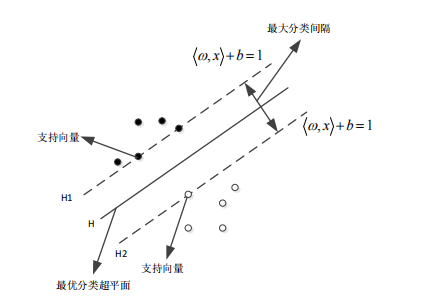
\includegraphics[width=0.5\textwidth]{svm.png}
	\caption{SVM模型原理图}
	\label{fig:svm}
\end{figure}

2、表模板
\begin{table}[htpb]
\caption{最优算法的多指标分析}
\begin{center}\label{table:score}
\begin{tabular}{|c|r|r|r|}
\hline
   & \multicolumn{1}{c|}{精确率} & \multicolumn{1}{c|}{召回率} & \multicolumn{1}{c|}{F1得分} \\ \hline
石块 & 0.94                     & 0.96                     & 0.95                      \\ \hline
金属 & 0.92                     & 0.97                     & 0.95                      \\ \hline
塑料 & 0.96                     & 0.89                     & 0.93                      \\ \hline
\end{tabular}
\end{center}
\end{table}

3、公式模板
\begin{equation}\label{eq:svmsuper}
\begin{array}{l}
\min _{\boldsymbol{w}, b} \frac{1}{2}\|\boldsymbol{w}\|^{2} \\
\text { s.t. } y_{i}\left(\boldsymbol{w}^{\mathrm{T}} \boldsymbol{x}_{i}+b\right) \geqslant 1, \quad i=1,2, \ldots, m
\end{array}
\end{equation}


4、伪代码模板
 \begin{algorithm}[H]
  \caption{ K近邻算法步骤}
  \begin{algorithmic}[1]
    \Require
      训练数据集;
      待预测数据;
    \Ensure
      预测数据的类别;
    \State 加载数据;
    \State 初始化K值;
    \State 计算预测样本与训练集中的每一个样本的距离;
    \State 将距离和索引添加到有序集合中;
    \State 对距离按从小到大排序方式对距离和索引的有序集合进行排序;
    \State 从排序的集合中选择前K条数据;
    \State 获得选的K条数据的标签;
    \State 计算每一种标签的样本数量;
    \Return 
        数量最多的标签作为样本的预测值;
  \end{algorithmic}
\end{algorithm}


5、代码模板
\lstset{language=Python}
\begin{lstlisting}
#调整图片尺寸到统一大小,并扁平化为一维数据
def image_to_feature_vector(image, size=(128, 128)):

	return cv2.resize(image, size).flatten()

#提取图像在HSV颜色空间上的颜色直方图,将直方图扁平化,
#作为特征向量返回
def extract_color_histogram(image, bins=(32, 32, 32)):
	hsv = cv2.cvtColor(image, cv2.COLOR_BGR2HSV)
	hist = cv2.calcHist([hsv], [0, 1, 2], None, bins,
		[0, 180, 0, 256, 0, 256])
	if imutils.is_cv2():
		hist = cv2.normalize(hist)
	else:
		cv2.normalize(hist, hist)
	return hist.flatten()

\end{lstlisting}
\end{appendices}

\end{document}
